%% Example data sheet
%% Feel free to modify and use this file for any purpose, under
%% either the LaTeX Project Public License or under public domain.

% Options here are passed to the article class.
% Most common options: 10pt, 11pt, 12pt
\documentclass[10pt]{datasheet}

% Input encoding and typographical rules for English language
\usepackage[utf8]{inputenc}
\usepackage[english]{babel}
\usepackage[english]{isodate}

% tikz is used to draw images in this example, but you can
% also use \includegraphics{}.
\usepackage{tikz}
\usepackage{pgfplots}
\usepackage{circuitikz}
\usetikzlibrary{calc}

% These define global texts that are used in headers and titles.
\title{MIPS CPU Data-sheet}
\date{December 2020}

\begin{document}
\maketitle

\section{Specification}


\begin{enumerate}
\item \textbf{Bus interface:} Instruction and data fetched over same interface allowing variable latency
\item \textbf{Avalon supported RAM}
\item \textbf{Supports 48 MIPS  instructions} 
\item \textbf{All signals are synchronous clock signals}
\item \textbf{Includes reset and halt behaviour:} 													Set high for at least 1 cycle , Active signal high.
\item \textbf{Two special memory locations:}											     	
\begin{itemize}
\item 0x00000000 : Attempt to execute address 0 causes CPU halt
\item 0xBFC00000 : Execution starts here after reset	

\end{itemize}
\end{enumerate}
 

\smallbreak

\section{Design Decisions}

\textbf{Multi cycle processor:} Chosen as was a necessary step to allow interaction with a non combinatorial memory and incorporate pipe lining into the design. Made usage of FSM imperative.

\textbf{Five stage pipeline:} Chosen to improve throughput, allowing five instructions to execute simultaneously. Increases the instructions per cycle (IPC) of the CPU up to 5x compared to a non-pipelined five stage MIPs CPU. Stages: Fetch , decode , execute , memory and write-back. Pipelining Demanded the use of a Hazard Unit to forward calculated register values which had not been written back to the register file yet. By splitting instructions into five stages, the critical path of the circuit was significantly reduced allowing for an increase in clock speed.

\textbf{Hazard handling:} Incorporated to handle hazards that occur when results of one in instruction are needed by a subsequent instruction before the latter has complete.

\section{Clever Features:}

\textbf{Branch prediction:} To maintain an average cycle per instruction (CPI) as close as possible to one, branch prediction is employed to reduce the number of pipeline flushes required for successful branch instructions.


\textbf{Sequential multiplier/divider: } This choice reduced the large area cost of combinatorial multiply and divide blocks whilst allowing for these operations to continue during unused Stall cycles. Further, it allowed for a higher frequency clock as the critical path was reduced.



{\textbf{Clock Gating}} 
The remove clock glitches between the master clock and the derived internal CPU clock, a latch was used to modify the clock enable line for the CPU on the negative half of the master clock cycle.

{\textbf{RAM State Machine}}
To communicate efficiently with RAM over the Avalon Bus interface a, six state finite state machine was employed to latch RAM data into CPU as well as stalling the CPU during a wait request.
\smallbreak


% Switch to next column

\section{Pin-out Diagram}

\smallbreak
\begin{figure}[h]
    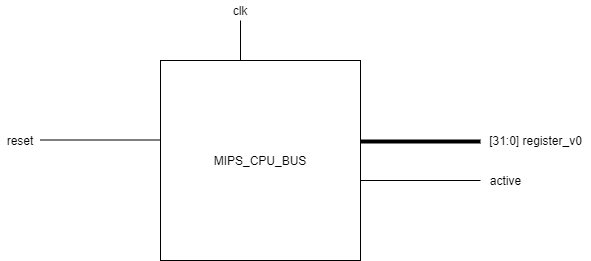
\includegraphics[scale=0.35]{Assets/bus.png}
\end{figure}



\section{Featured Components}
\textbf{Register File:} Holds data for 32 x 32 bit registers and two special HI and LO registers.

\textbf{ALU:} Executes arithmetic and logical operations.

\textbf{Program counter register:} Stores address of instruction to read from memory

\textbf{Branch Adder:} Computes the branch target address.

\textbf{Sign Extend:} Used to extend I-Instruction offset stored in immediate field. 

\textbf{Branch Comparator:} Determines if the branch instruction condition is successful, employed to perform branch prediction.

\textbf{Forwarding Mux:} Driven by the hazard unit, allowing calculated values which have not been written to the register file, be forwarded to the ALU.

{\textbf{Pipeline Registers}} Stores instruction data and control signals between pipeline stages.

\newpage

\onecolumn

\section{Architecture Overview}

\subsection{Data path}
The Data path consists of five stages separated by four pipeline registers (In the case of the Fetch and Memory stages no register is required as we interact with a sequential memory that operates under clocked operation already). Each stage has a major component and a number of minor components that dictates its operation and ensure correct function. These components are:

\begin{multicols}{2}

\textbf{Fetch Stage:} Memory (Instruction memory), Program Counter Register , PC increment , PC Mux 

\textbf{Decode Stage:} Register File, Sign Extend , Bit Shift , Branch Adder , Comparator , Forwarding Muxs.

\textbf{Execute Stage:} ALU, Forwarding Muxs, Register Destination Mux , ALU Src Mux.

\textbf{Memory Stage:} Memory (Data Memory),

\textbf{Write-back stage:}Register File, Memory to Reg Mux.

\end{multicols}

\subsection{Control unit}
The control unit produces control signals during the decode stage by examining the \textit{opcode} and \textit{funct} fields of an instruction.The incorporation of pipe-lining made it so that all signals associated with one instruction must advance through the pipeline in unison with said instruction to remain synchronised with the instruction they are associated, ensuring correct operation. 



\subsection{Hazard unit} 
Prevents  RAW hazards that occur when instructions are dependant on results of another instruction through forwarding and stalling. Prevents Control hazards through flushing and stalling CPU operations. With a combinatorial block that accesses a number of component control lines.




\begin{figure}[h]
    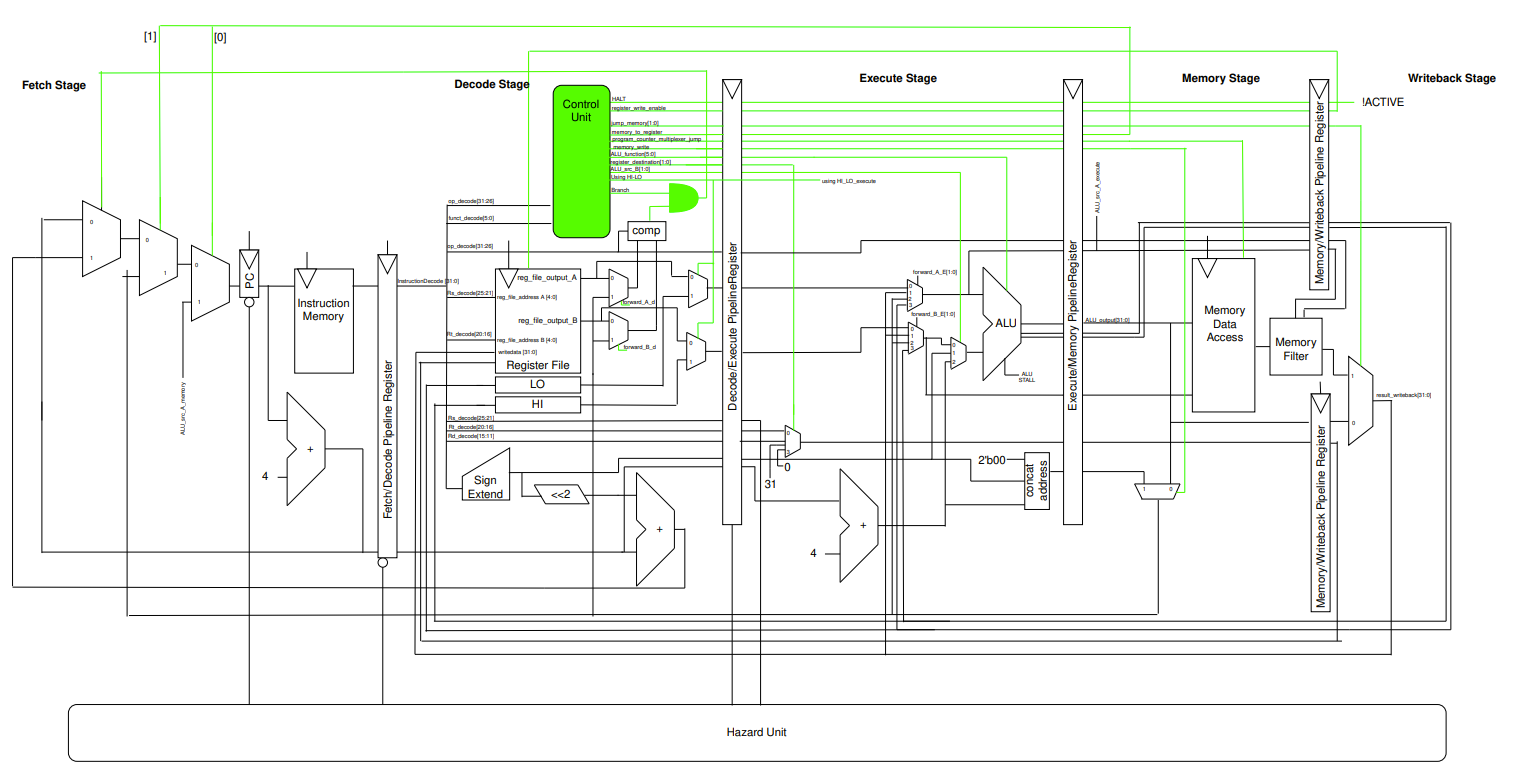
\includegraphics[scale=0.75]{Assets/circuit.PNG}
    \centering
    \captionsetup{justification=centering}
    \caption{Overview of Architecture}
\end{figure}


\newpage

\twocolumn

\section{Testing Approach}
\smallbreak
Testing was performed by two separate methodologies, one methodology tested the full architecture from ground up focusing on architecture robustness whilst a second tested for functional correctness using CPU I/O (as a third party would). This distinction ensured the testing was not designed to solely evaluate our architecture but could also be used on similar MIPS architectures. Further it prevented any framing or confirmation bias in evaluation of results.
\smallbreak

Each component varies in functionality and make up so testing was tailored for each component / block , the table highlights the test strategy used on each.

\begin{figure}[h]
    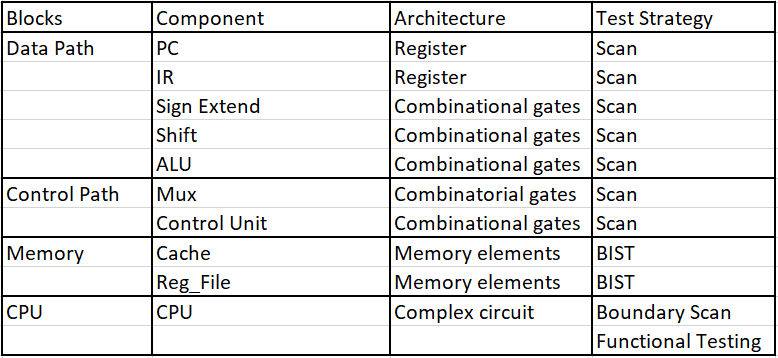
\includegraphics[scale=0.7]{Assets/Strategy.PNG}
    \captionsetup{justification=centering}
    \caption{Test Strategy table}
\end{figure}

\smallbreak


\textbf{Methodology one} (Robustness Testing): Performed all logic scan , BIST and boundary scan testing through the development of our architecture. This testing occurred in an order determined by the component hierarchy. Testing begins at each bottom component and moves up the hierarchy, testing intermediate circuity as it continues. 
\smallbreak

\begin{figure}[h]
    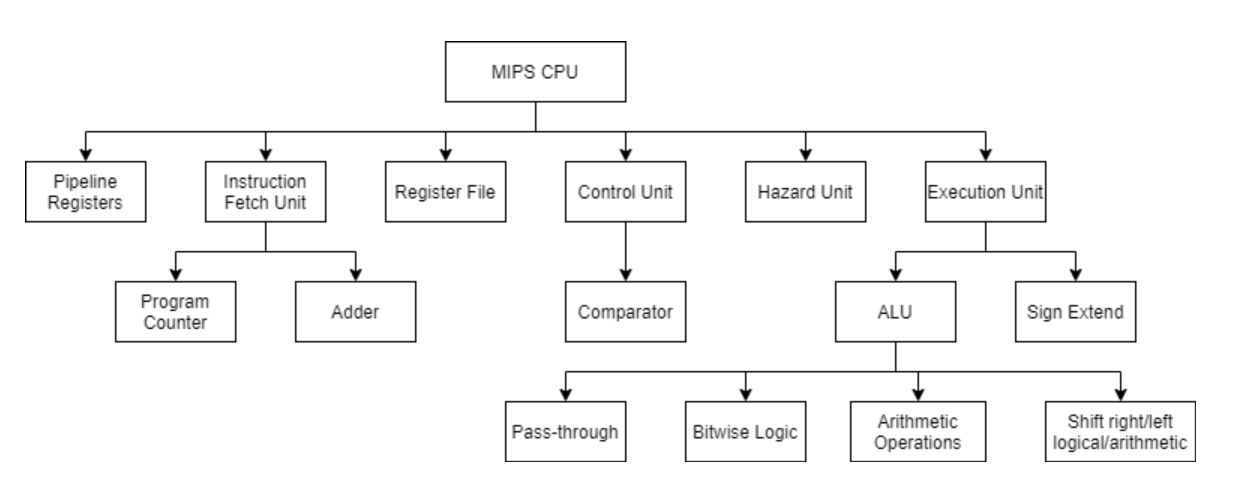
\includegraphics[scale=0.45]{Assets/hierarchy2.png}
    \captionsetup{justification=centering}
    \caption{CPU Component Hierarchy}
\end{figure}

\smallbreak

Component testing method:

1. Identify inputs, outputs and intended behaviour

2. Using verilator write cpp code, feeding the module with different inputs and checking outputs manually or automatically.
Manual: values chosen by hand to see how the module handles certain edge cases.Automatic: values chosen 'randomly' (on a set increment or by multiplying increments).

\vfill\break

3. If a test case fails, log information usually inputs, expected value, returned value and any other outputs from the module.

 



\textbf{Methodology Two} (Functional Testing): Utilises a virtual RAM to control inputs to the CPU and as such, tests individual and combinations of instructions. Again it follows a ground up approach testing the least logically and architecturally complex instructions first. R-Type instructions (aside from 3 shift instructions) only use registers in their operation so were tested first. Followed by J-Type then I-Type.

\begin{figure}[h]
    \centering
    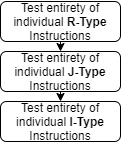
\includegraphics[scale=0.7]{Assets/functionalflow (1).PNG}
    \captionsetup{justification=centering}
    \caption{Functionality testing flowchart}
\end{figure}

\textbf{Method of testing for instructions and programs:}

The test bench employs a MIPS parser which produces a hex file of a test case regarding a certain instruction. Each test case consists of a comment regarding the instruction to be tested, the index of the test case, the expected output in register v0, and any additional notes. The RAM is then initialised with the HEX file and linked with the CPU to simulate the test case. The test bench then compares the output in register v0 with the expected output in the comment, to produce the final outcome giving information regarding the pass or fail of the instruction.

\textbf{Instruction Tests}: Each instruction was tested by 2 to 5 test cases designed to test normal and extreme operation. It began by testing simple cases and progressed to edge cases involving interactions with multiple instructions, extreme inputs / outputs and extreme memory access

The functional testing methodology was designed to test any MIPS ISA using a range of software testing principles. Unit testing was performed in the early instruction tests where each instruction of the ISA was scrutinised. Integration testing was performed in the later edge case tests where we ensured good collaboration of instructions. This ensured a holistic and specialised testing approach. 


\smallbreak



\onecolumn

\section{Area and timing summary}
\smallbreak

\begin{table}[h]
\caption{\textbf{Timing Specifications Summary } }
\begin{tabularx}{\textwidth}{l | c | c |  X}
    \thickhline
    \textbf{Parameter} &  \textbf{Fmax} & \textbf{Unit} & \textbf{Conditions} \\
    \hline
    Maximum clock frequency  & 42.17 & MHz & 1200mV 85C \\
     \hline
    Maximum clock frequency  & 37.25 & MHz & 1200mV 0C \\
    \thickhline
\end{tabularx}
\footnotetext[1]{Based on characterization data, not tested in production.}
\end{table}

Analysis showed that the Worst-Case Timing Paths: \verb|Decode_Execute_Register| \verb|->| \verb|ALU_Multiplier|

\begin{table}[h]
\caption{\textbf{Area Specifications Summary } }
\begin{tabularx}{\textwidth}{l | X}
    \thickhline
    \textbf{Parameter} &  \textbf{No.} \\
    \thickhline
    Total Logic Elements &  6,595\\
    \hline
    Combinatorial w/ no register  & 4,236  \\
     \hline
    Register only & 192  \\
    \hline
    Combinatorial w/ register & 2,167 \\
    \hline
    Total registers & 2,359 \\
    \thickhline
\end{tabularx}
\footnotetext[1]{Based on characterization data, not tested in production.}
\end{table}

\begin{table}[h]
\caption{\textbf{Power Specifications Summary } }
\begin{tabularx}{\textwidth}{l | c | X}
    \thickhline
    \textbf{Parameter} & \textbf{Value} &  \textbf{Unit} \\
    \thickhline
    Total Thermal Power Dissipation & 158.77 & mW\\
    \hline
     Core Dynamic Thermal Dissipation  & 41.23 & mW  \\
     \hline
    Core Static Thermal Dissipation & 50.41 & mW  \\
    \hline
    I/O Thermal Dissipation & 67.13 & mW  \\
    \thickhline
\end{tabularx}
\footnotetext[1]{Based on characterization data, not tested in production.}
\end{table}
Power - Low Estimation Confidence.

\textbf{Note:} All measurements taken above were performed in the Cyclone IV E Auto Quartus

\end{document}


